\section{Routing Protocols}

% \begin{figure*}[!t]
% 	\centering
% 	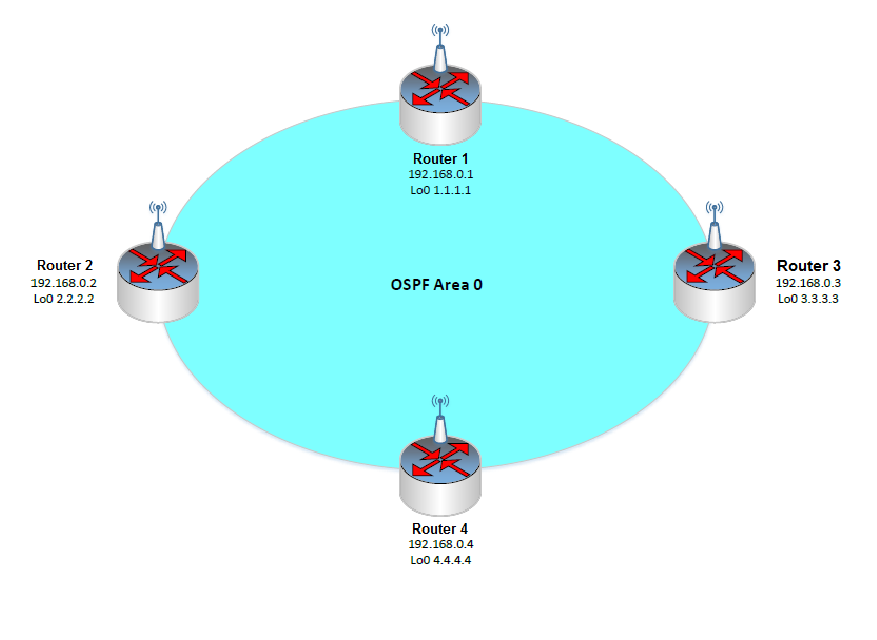
\includegraphics[width=0.7\textwidth]{figs/topology.eps}
% 	\caption{Wireless Network topology.}
% 	\label{Fig01}
% \end{figure*}

Traditional mesh routing solutions have focused on simply finding the best route to the gateway to reach the Internet. Two important underlying assumptions of these routing solutions are: 1) all gateway nodes are equally capable in terms of resources such as bandwidth capacity and delay to connect to the Internet; and/or 2) the capacity bottleneck is in the wireless multihop portion of the WMN \cite{Prashanth2015}.

% Due to the severe energy constraints of large number of densely deployed sensor nodes, it requires a suite of network protocols to implement various network control and management functions such as synchronization, node localization, and network security. The traditional routing protocols have several shortcomings when applied to WSNs, which are mainly due to the energy-constrained nature of such networks \cite{Shio2010}.

OSPF is one of the most studied and well-known link state routing protocols to date. Being a link state protocol, every router maintains a complete map of the network topology. Consequently, at any given moment a router can compute the path to any destination in the network, based on its existing knowledge about the network \cite{Holter2010}.

\section{Environment Sensor System}
In many WSN applications, the deployment of sensor nodes is performed in an ad hoc fashion without careful planning and engineering. Once deployed, the sensor nodes must be able to autonomously organize themselves into a wireless communication network. Sensor nodes are battery-powered and are expected to operate without attendance for a relatively long period of time \cite{Shio2010}.

Computers have to be kept in a specific environment to function efficiently. Conditions such as heat, cold, dust and excessive humidity all can damage and lessen the performance of a computer. External and internal temperature especially causes fluctuations of performance, although a computer is more vulnerable to heat than to cold.

\subsection{Temperature}
\subsubsection{Overheating}
Electronic devices are vulnerable to overheating. The electronic components operate at a specific current induced by a voltage. The sensitivity of the components means that even a small fluctuation in voltage is dangerous. Excessive heat lowers the electrical resistance of objects, therefore increasing the current. In addition, slowdown is a result of overheating. Components can shut down when overheated.

\subsubsection{Cold Temperatures}
Cold temperatures are not as dangerous to a electronic devices as overheating is, but problems can still occurs. If Electronic devices get too cold when left powered off, their components can be damaged upon boot because the electricity heats the circuit. As electricity travels through a circuit, it heats rapidly and causes the matter to expand. Rapid expansion, when close to matter that remains the same size, it distorts it. This can bend or break component.

\subsubsection{Ideal Operating Temperatures}
Semiconductor parts are most often specified for use in the “commercial” 0 to 70°C and, to a lesser extent, in the “industrial” -40 to 85°C operating temperature range. These operating temperature ratings generally satisfy the demands of the dominant semiconductor customers in the computer, telecommunications, and consumer electronic industries \cite{Mishra2004}.

\subsection{Humidity}
Excessive humidity or dry air can exaggerate the effects of extreme temperatures on computer components. For example, dry air causes static electricity to build up. Coupled with the increased conductivity from heat, this can cause errant discharges. Conversely, cold and humid areas create condensation and water, which can create a short circuit.

\subsection{Luminosity}
In the wireless sensor network context, the luminosity factor may be extremely decisively, once the network nodes are generally supplied by batteries that can be recharged by solar panels.

\section{Context-aware routing}
The Reconfiguration Manager performs cross-layer context monitoring throughout the system and reorganizes, in co-ordination with the Context Source Manager, the mappings between context fact types in the context models and appropriate sources. This is the component in ACoMS that delivers its self-healing capabilities.

% TODO
% \subsubsection{Environment context Criteria Decision}

% \subsection{Hardware select} % (fold)
% \label{sub:hardware_select}

%% ------------------   Traduzir   ------------------

\subsubsection{DHT11: Humidity and Temperature Sensor}

DHT11 is a humidity and temperature sensor that can read temperatures between 0 and 50 Celsius degrees and humidity between 20 and 90\%.

\begin{figure}[h]
\centering

    \begin{subfigure}[b]{0.2\textwidth}
		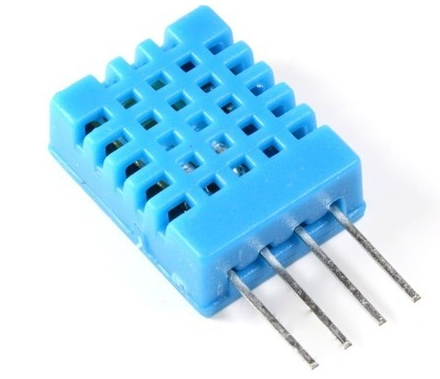
\includegraphics[width=\textwidth]{figs/dht11}
		\caption{DHT11 view}
		\label{fig-dht11}
    \end{subfigure}
    %
    \begin{subfigure}[b]{0.2\textwidth}
	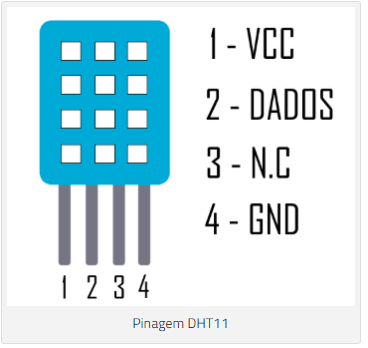
\includegraphics[width=\textwidth]{figs/dht11-pinagem}
	\caption{DHT11 pins}
	\label{fig-dht11-1}
    \end{subfigure}
	\caption{DHT11 sensor}
\end{figure}

The temperature value is measured by an NTC thermistor (Negative Temperature Coefficient-thermistors: the resistance lowers with the increase of the temperature) and the relative humidity through a capacitive sensor. \cite{robotics2010dht11}. Fig. \ref{fig-temp-data} shows an example of temperature data read using the DHT-11 by one of the network routers.

\subsubsection{Luminosity sensor: LDR(Light Dependent Resistor)}

The LDR (Light Dependent Resistor) has a characteristic that makes its resistance vary according to the environment luminosity. This enables the use of this component to develop a sensor that is activated (or deactivated) when a certain luminosity threshold is reached.

\begin{figure}[!tb]
\centering
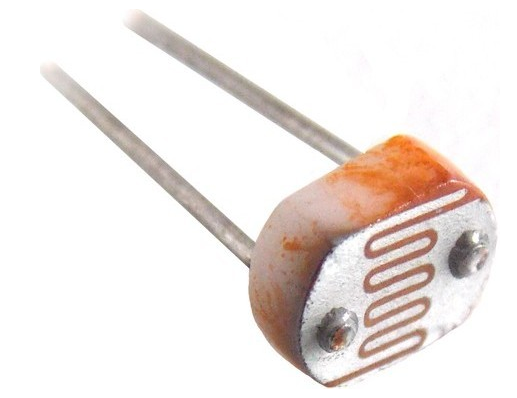
\includegraphics[width=0.38\textwidth]{figs/ldr}
\caption{LDR sensor}
\label{fig-ldr}
\end{figure}

The resistance of the LDR varies inversely to the amount of light incident on it. While the beam of light is falling on it, the LDR offers a very low resistance, and when this beam is cut, its resistance increases \cite{ldr2010manual}. Fig. \ref{fig-ldr-data} shows an example of data read using the LDR by one of the network routers.

\begin{figure}[!tb]
\centering
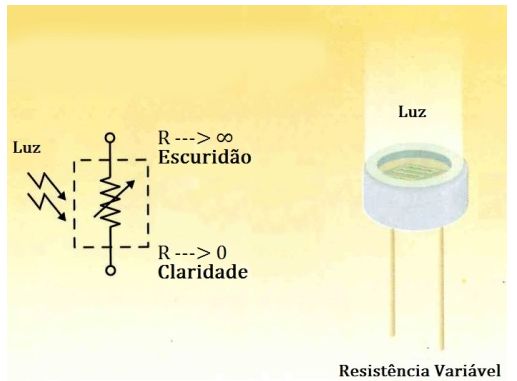
\includegraphics[width=0.38\textwidth]{figs/ldr-1}
\caption{LDR sensor use}
\label{fig-ldr-1}
\end{figure}


%% ------------------   Traduzir   ------------------

% ../externos/dados/LDR.csv

\begin{figure}[!tb]
  \begin{center}
    \begin{tikzpicture}
      \begin{axis}[
          width=\linewidth, % Scale the plot to \linewidth
          grid=major, 
          grid style={dashed,gray!30},
          % xlabel=X Axis $U$, % Set the labels
          ylabel=Light,
          % x unit=\si{\volt}, % Set the respective units
          % y unit=\si{\ampere},
          legend style={at={(0.5,-0.2)},anchor=north},
          x tick label style={rotate=90,anchor=east}
        ]
        \addplot 
        % add a plot from table; you select the columns by using the actual name in
        % the .csv file (on top)
        table[x=x,y=light,col sep=comma] {../externos/dados/LDR.csv}; 
        % \legend{Plot}
      \end{axis}
    \end{tikzpicture}
    \caption{Light read from sensor}
    \label{fig-ldr-data}
  \end{center}
\end{figure}

\begin{figure}[!tb]
  \begin{center}
    \begin{tikzpicture}
      \begin{axis}[
          width=\linewidth, % Scale the plot to \linewidth
          grid=major, 
          grid style={dashed,gray!30},
          % xlabel=X Axis $U$, % Set the labels
          ylabel=Temperature,
          % x unit=\si{\volt}, % Set the respective units
          % y unit=\si{\ampere},
          legend style={at={(0.5,-0.2)},anchor=north},
          x tick label style={rotate=90,anchor=east}
        ]
        \addplot 
        % add a plot from table; you select the columns by using the actual name in
        % the .csv file (on top)
        table[x=x,y=temperature,col sep=comma] {../externos/dados/DHT.csv}; 
        % \legend{Plot}
      \end{axis}
    \end{tikzpicture}
    \caption{Temperature read from sensor}
    \label{fig-temp-data}
  \end{center}
\end{figure}

\begin{figure}[!tb]
  \begin{center}
    \begin{tikzpicture}
      \begin{axis}[
          width=\linewidth, % Scale the plot to \linewidth
          grid=major, 
          grid style={dashed,gray!30},
          % xlabel=X Axis $U$, % Set the labels
          ylabel=Humidity,
          % x unit=\si{\volt}, % Set the respective units
          % y unit=\si{\ampere},
          legend style={at={(0.5,-0.2)},anchor=north},
          x tick label style={rotate=90,anchor=east}
        ]
        \addplot 
        % add a plot from table; you select the columns by using the actual name in
        % the .csv file (on top)
        table[x=x,y=humidity,col sep=comma] {../externos/dados/DHT.csv}; 
        % \legend{Plot}
      \end{axis}
    \end{tikzpicture}
    \caption{Humidity read from sensor}
  \end{center}
\end{figure}

\begin{figure}[!tb]
\begin{center}\begin{circuitikz} 
  % (0,0) to [pDo=$R_1$,*-*] (3,3)
  % (0,0) to [R=$R_3$,*-*] (3,-3)
  % (3,-3) to [R=$R_x$,*-*] (6,0)
  % (3,3) to [R=$R_2$,*-*] (6,0)
  % (0,0)to[ammeter] (6,0)
  % (3,-3) node[ground] {};
  % \draw (3,3) -- node[] {} (3,3.5);
  % \draw (2.5,3.5) --  node[anchor=south] {VCC} (3.5,3.5)  node[anchor=west] {};
  % \draw (0,0) node[anchor=east]{$A$};
  % \draw (6,0) node[anchor=west]{$B$};

  \draw (0,0) -- (0,2) to [R=10<\kilo\ohm>,*-*] (2,2);
  \draw (0,2) -- (0,3) to [R=10<\kilo\ohm>,*-*] (2,3);
  \draw (0,3) to[short,*-o] (0,5) node[above]{$V_{CC}=3.3V$}; % Power supply
  \draw (0,4) to[short,*-] (1.9,4) -- (1.9,4.5);
  \draw (0,0) to [pDo,*-*](2,0) to [eC,l=10<\micro\farad>,*-*](4,0) -- (4,4) -- (2.2,4) -- (2.2,4.5);
  \draw (4,3.5) to[short,*-] (4.5,3.5) node[ground]{};
  \draw (2,2) -- (2,4.5);
  \draw (2.1,4) -- (2.1,4.5);
  \draw (1.4,5.7) rectangle (2.7,4.5)
    node at(2.05,5.1){DHT11};
   %gpio pins
  \draw (2,0) to[short,*-o] (2,-1) node[right]{Pin11};
  \draw (2,2) to[short,*-o] (2.5,2) node[right]{Pin7};

 \end{circuitikz} \end{center}
\caption{Sensor circuit}
\label{ponte}
\end{figure}

